%----------------------------------------------------------------------------
\chapter{Hallgatói értékelési rendszer}\label{chapter:assessments}
%----------------------------------------------------------------------------

A korábban leírtaknak megfelelően a JPorta tárgyaiban lehetőség van különböző értékeléseket felvenni, majd azokat kurzusokhoz rendelni. Ezeket hozzárendelés után a kurzus oktatói tudják értékelni (\ref{fig:jporta_course_results}. ábra).

Új értékelést csak a tárgy adminisztrátorai tudnak létrehozni és kurzusokhoz rendelni. Az ehhez tartozó felület \aref{fig:jporta_add_result}. ábrán látható. Minden értékeléshez az alábbi tulajdonságok tartoznak:
\begin{itemize}
    \item Név: rövid név, mely azonosítja az értékelést, pl. ZH 1
    \item Típus: előre definiált értékek, melyekhez tartozik egy reguláris kifejezés \cite{RegExp}. Csak olyan értéket vehet fel, ami illeszkedik a hozzá tartozó kifejezésre.
    \item Súly: meghatározza a sorrendet az értékelések megjelenítésénél.
    \item Ki értékelheti: kurzusokhoz, vagy csak a tárgyhoz rendelt oktatók értékelhetik.
    \item Dinamikus-e: az adott értékelés dinamikusan értékelődik-e ki, ld. \aref{section:dynamic-assessments} pontban.
    \item Privát-e: a privát értékeléseket csak az oktatók látják, a hallgatók nem.
    \item Megjegyzés: részletes leírása az értékelésnek, tipikusan dinamikus értékelések esetén hasznos.
    \item Kurzusok: tárgyon belül mely kurzusokhoz akarjuk hozzárendelni az értékelést.
\end{itemize}

\begin{figure}[h]
    \centering
    \resizebox{\textwidth}{!}{
        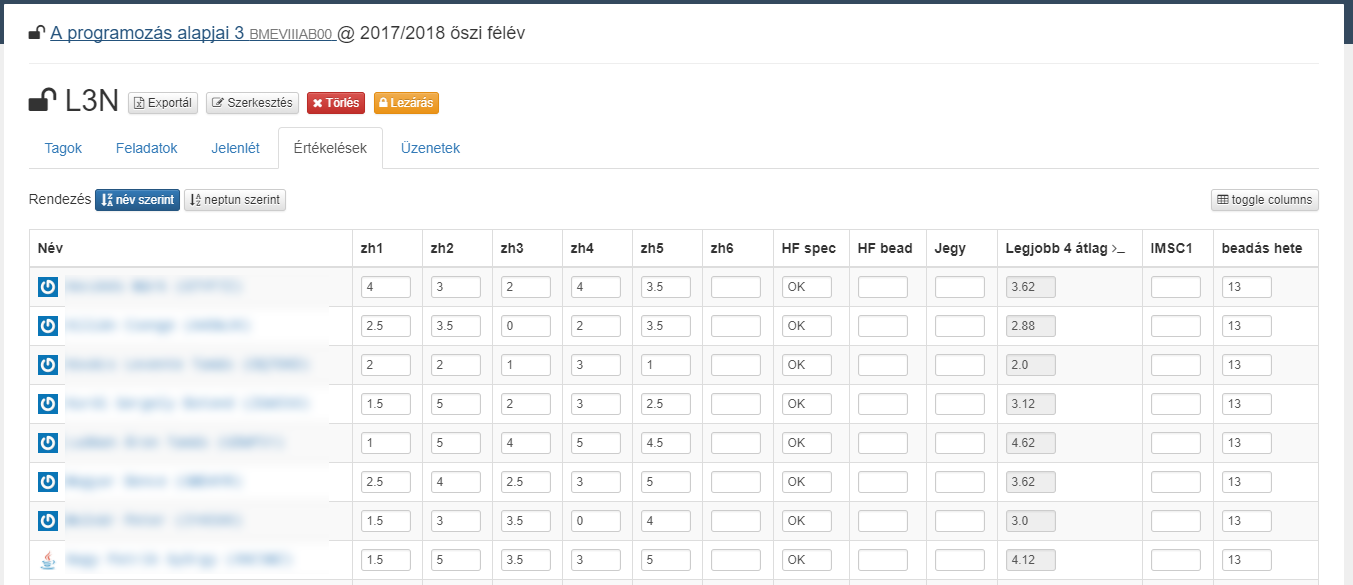
\includegraphics[]{jporta_course_results.png}
    }
    \caption{Hallgatók értékelései}
    \label{fig:jporta_course_results}
\end{figure}

Ezen tulajdonságoknak köszönhetően az értékeléseket egyszerűen és személyreszabhatóan lehet kezelni. Alapvető céljuk a zárthelyi számonkérések eredményének adminisztrálása, de bármikor hozzáadhatunk egyéb mezőket is. Ilyen lehet pl. a hallgató házi feladatának személyes bemutatására kijelölt időpont, vagy éppen a házi feladat dokumentáció státusza.

Az univerzalitás egyedüli határa a megfelelő típus megtalálása az értékeléshez, de ez könnyen bővíthető. Új igény felmerülésekor a portál adminisztrátorai hozzáadhatnak új típust, mely egy tetszés szerinti reguláris kifejezésre illeszkedő tartalmat vár.

\begin{figure}[p]
    \centering
    \resizebox{0.9\textwidth}{!}{
        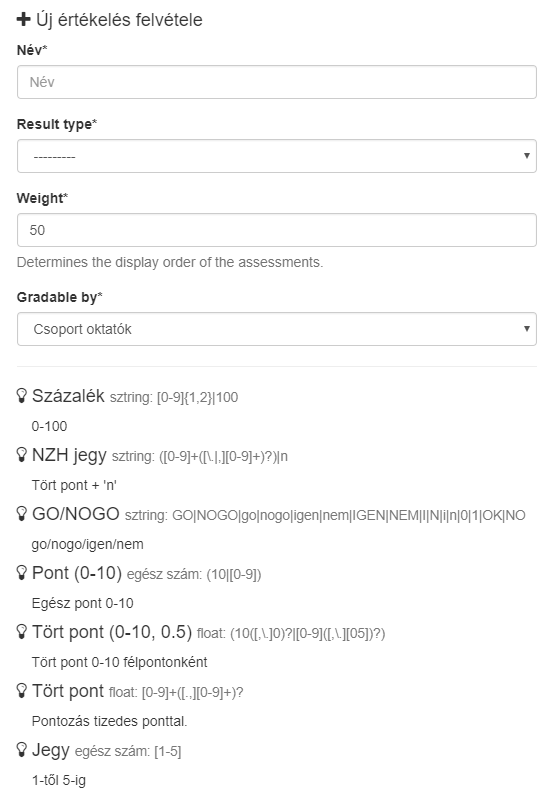
\includegraphics[]{jporta_add_result.png}
    }
    \caption{Értékelés típus hozzáadása}
    \label{fig:jporta_add_result}
\end{figure}

\section{Dinamikus értékelések}\label{section:dynamic-assessments}

Az értékelések létrehozásánál hamar felmerült az igény a dinamikus, azaz automatikusan számolódó mezők használtára. Ezek nagyban megkönnyítik a félév végi összesítést és a végső jegy meghatározását. Viszont ahhoz, hogy ezt széleskörűen lehessen használni egy teljesen általános rendszert kellett fejleszteni, hiszen minden tárgynak eltérő, akár félévről félévre változó követelményei lehetnek, melyekhez más és más számolásokat, súlyozásokat kellhet végezni. 

Ennek megoldására a jelengi implementáció előtt is volt mód, ám az fapadosnak számított. Először az oktatóknak exportálni kellett a meglévő eredményeket egy Excel fájlba, majd ezt a fájlt külső programmal szerkesztve kellett létrehozniuk a dinamikus mezők értékeit. Csak ezután tölthették fel a portálra a bővített fájlt, melynek feldolgozása során a JPorta az ebben található értékeket frissítette. Ezt a módszert Kálmán Viktor cserélte le a jelenlegi alternatívára \cite{KalmanMsc}.

\section{Dinamikus értékelések jelenlegi implementációja}\label{section:dynamic-assessments-impl}
Az aktuális megvalósításnak két fő követelményt támasztottak: webes felületen beállíthatónak és az oktatók számára könnyen testreszabhatónak kellett lennie.

Ezek teljesítése érdekében a dinamikus mezők kiszámolására Python nyelven írt kódokat használ a portál. Minden dinamikus mezőhöz webes felületen módosítható kód tartozik, amely megkapja a hallgatókhoz tartozó adatokat, majd ez alapján kiszámolja a mező értékét. A megadott Python kódnak tartalmaznia kell egy \textit{calculate\_result} függvényt, mely három szótár (dictionary) típusú paraméterrel rendelkezik:

\begin{enumerate}
    \item paraméter a jelenléteket tartalmazza külön előadás, laboratóriumi és gyakorlati órákra bontva. Minden típushoz megtalálható, hogy hány alkalommal volt jelen a hallgató (attended), hány alkalommal lett megtagadva a jelenléte (denied), hány alkalommal nem jelent meg (no), illetve hogy összesen hány foglalkozás volt tartva abból a típusból (all).
    \item paraméter a (nem dinamikus) értékeléseket taralmazza, \textit{None} értéket ott, ahol nincs megadva eredmény. A kulcs mindig az adott értékelés azonosítója.
    \item paraméterben pedig az automatikusan kiértékelődő feladatok eredményei találhatóak. A kulcs itt is mindig az adott feladat azonosítója, értékei pedig az alábbiak: 
    \begin{itemize}
        \item \textit{None}, ha az adott feladatra nem adott be megoldást a hallgató.
        \item \textit{0}, ha az adott feladat kiértékelés alatt van.
        \item \textit{1}, ha az adott feladat oktatói jóváhagyásra vár.
        \item \textit{2}, ha az adott feladat sikertelen.
        \item \textit{3}, ha az adott feladat sikeresen lefutott.
    \end{itemize}
\end{enumerate}

Ez a függvény minden hallgatóra egyesével fog meghívódni, visszatérési értéke pedig megadja a mező értékét az adott hallgatónál.

Az alábbi példa kód a Programozás alapjai 3. tárgynál használt egyik dinamikus mezőhöz tartozik, feladata a félév végi átlag kiszámítása. Itt a félév során megírt 6 db zárthelyi dolgozatból a legjobb 4 átlagát kell venni, majd kerekíteni 2 tizedesjegyre. A további kerekítést a laborvezető oktatók végzik.

\begin{lstlisting}
def calculate_result(atds, asms, asgs):
    results = [asms[374], asms[375], asms[376], asms[377], asms[378], asms[379]]
    results = [x for x in results if x is not None]
    results.sort(reverse=True)
    return round(sum(results[:4])/4, 2)
\end{lstlisting}

Természetesen a kötelező \textit{calculate\_result} függvény mellett tetszőleges számban használhatunk segédfüggvényeket is a számolás átláthatósága és egyszerűsítése érdekében.

\section{Dinamikus értékelések tesztelése}
Az így elkészített dinamikus mezőben könnyen előfordulhatnak programozói hibák, emiatt a kód felhasználása előtt elengedhetetlen annak átfogó tesztelése. Szerencsére a korábban elkészült rendszer ezt is támogatja. \Aref{fig:jporta_dynamic_test}. ábrán látható módon meg tuduk adni teszt bemeneti paramétereket, majd a rendszer (az eredeti kiértékeléssel megegyező módon) kiszámolja a dinamikus mezőhöz tartozó értéket, így meggyőződhetünk a helyes működéséről.

\begin{figure}[h]
    \centering
    \resizebox{\textwidth}{!}{
        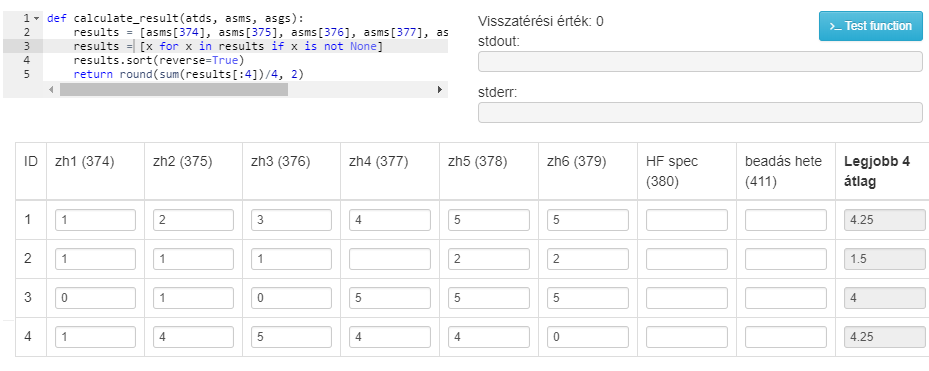
\includegraphics[]{jporta_dynamic_test.png}
    }
    \caption{Dinamikus mező tesztelése}
    \label{fig:jporta_dynamic_test}
\end{figure}

Az értékek mellett láthatjuk a programunk kimeneteit és visszatérési értékét is. Ezeket akár a teszteléshez is felhasználhatjuk, azonban élesítés előtt célszerű ezeket törölni, mivel a portál minden éles futásról tárolja az ilyen jellegű adatokat az ellenőrizhetőség miatt.

Ugyan a példában nem volt szükség sem a jelenlétekre, se az automatikusan kiértékelődő feladatok eredményére, ezeket a számonkérésekhez hasonlóan fel tudjuk használni, illetve a tesztelés is az előzőekkel megegyezően működik.

\section{Dinamikus mezők dinamikus függőségei}\label{section:dynamic_dependencies}
Ez a rendszer az alapvető igényeket ugyan kielégíti, de hamar felmerült két fő hiányossága:

\begin{itemize}
    \item Dinamikus mezők kiszámítására nem használhatunk más dinamikus mezőket. 
    \item Jelenleg nem lehet egy hallgatóra vagy kurzusra újraszámolni a dinamikus mezők értékeit, hanem mindig a tárgy összes hallgatójára újra kiértékelésre kerülnek ezek. Kezdetben ez nem tűnt nagy pazarlásnak, mivel 10-20 másodpercnél többet nem vesz igénybe a művelet egy 400 fős tárgy esetében \cite{KalmanMsc}, azonban felhasználva az előző pont miatt szükséges módosításokat, már sokkal közelebb kerülünk ennek a pontnak a megoldására is.
\end{itemize}

Az első hiányosság miatt, ha egy tárgy esetében szeretnénk, hogy a hallgatók láthassák külön a zártyhelyi dolgozataik átlagát, majd ezen érték és más mezők alapján egy másik mezőt is hozzá szeretnénk adni, akkor ezt csak kódduplikációval tehetjük meg. Azaz mindkét mezőnél meg kell adnunk ugyan azt a Python kód részletet, illetve a második mezőnél ezt még ki kell egészítenünk. Ez számos problémát felvet: a kód nem újrahasználható, módosítások hibalehetőséget rejtenek, illetve akár inkonzisztens értékeket is előállítatunk, ha a kódokat nem sikerül szinkronban tartani.

A szakdolgozatom keretében erre a problémára is kerestem a megfelelő megoldást, melyet két kulcsfontosságú részre bontottam: függőségek meghatározása, majd ezek alapján a függőségi gráf kiértékelése.

A függőségek meghatározására több módszert is megvizsgáltam. Végül amellett döntöttem, hogy a felhasználóknak kell megadniuk, mely dinamikus mezőket szeretnék használni (ld. \ref{fig:jporta_dynamic_dependencies}. ábra). Ennek előnye, hogy egyszerű meghatázorni a függőségeket (hiszen a felhasználó explicit megadja azokat), hátránya pedig, hogy külön beállítást igényel. Az automatikus függőség felismeréshez szükséges lett volna a mezőhöz tartozó Python kód elemzése, mely értékéhez mérten aránytalanul sok időráfordítást követelt. Emiatt döntöttem a másik megoldás mellett. Ezen információk birtokában pedig bármelyik értékeléshez előállítható a teljes függőségi gráf egy egyszerű rekurzív bejárással.

\begin{figure}[h]
    \centering
    \resizebox{\textwidth}{!}{
        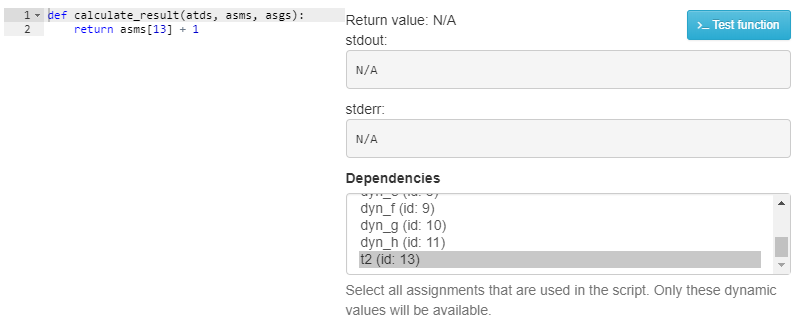
\includegraphics[]{jporta_dynamic_dependencies.png}
    }
    \caption{Dinamikus értékelés függőségkezelés}
    \label{fig:jporta_dynamic_dependencies}
\end{figure}

Minden függőségnek jelölt mezőt a többi értékeléssel együtt lehet felhasználni, \aref{section:dynamic-assessments-impl}. pontban leírt módon. Így nem kellett módosítani a jelenlegi függvény paraméter listát, illetve a logikailag összetartozó részek hasonlóan érhetőek el.

Külön figyelmet kellett fordítani a körkörös függőségek felderítésére, mivel ezek kiértékele végtelen ciklust eredményezne. Annak érdekében, hogy az adatbázisba ne kerülhessen körkörös függőség, ezt még a mentés előtt ellenőrzöm. Megvizsgálom, hogy a megjelölt függőségek közül van-e olyan, ami az aktuálisan módosított példánytól függ. Ha létezik ilyen, akkor ez egy körkörös függőség.

A másik rész a függőségi gráf kiértékelése volt. Dinamikus függőségek nélkül a sorrend nem befolyásolja a végeredményt, azonban ezen megkötések mellett már nem minden sorrend fog helyes eredményt adni. 

\Aref{fig:dependency_graph}. ábrán láthatunk egy példa függőségi gráfot, ahol 
\begin{itemize}
    \item $a \rightarrow b$ jelenti $a$-nak $b$-től való függőségét,
    \item a folytonos elipszis jelenti, hogy az adott dinamikus értékelés kurzushoz van rendelve, azaz kötelező kiszámolnunk az értékét,
    \item a szaggatott elipszis jelenti, hogy az értékelés nincs kurzushoz rendelve, azaz az értékét nem kötelező kiszámolni, ha más nem hivatkozik rá.
\end{itemize}

\begin{figure}[h]
    \centering
    \resizebox{0.8\textwidth}{!}{
        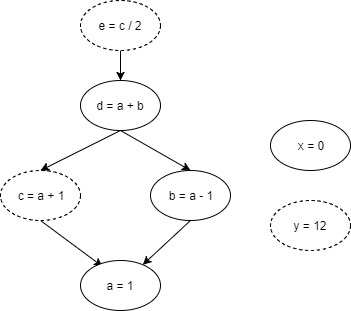
\includegraphics[]{dependency_graph.png}
    }
    \caption{Függőségi gráf}
    \label{fig:dependency_graph}
\end{figure}

Mivel a függőségek kialakításánál csak az irányított körmentesség a feltétel, kialakulhatnak különböző összefüggő komponensek és izolált pontok. Ezek közül csak azokat akarjuk kiértékelni, melyekre valóban szükség is van, azaz vagy hozzá van rendelve kurzushoz, vagy valamelyik kurzushoz rendelt mező (közvetlen vagy közvetett) függősége.

Ezek értelmében pl. az $a, b, c, d, x$ kiértékelési sorrend megfelelő eredményt ad, mivel minden elem kiértékelésekor azok függőségeit már kiértékeltük és pontosan azokat a mezőket vettük bele a sorrendbe, amelyekre szükségünk van.

A sorrend előállításához először felépítettem egy függőségi gráfot minden olyan elemből kiindulva, mely kurzushoz van rendelve. Minden így megtalált függőséget hozzáadtam a gárfhoz és rekurzívan megvizsgáltam az ahhoz tartozó függőségeket, ha az még nem létezett a gárfban. Ennek eredményeként előállt a függőségi gráf, mely pontosan a szükséges elemeket tartalmazta.

Ez alapján a sorrend felállításához felhasználtam Dudás Ádám a JPorta más részein is használt ütezemőjét \cite{DudiMsc}. Ez a megoldás egy függőségi gráf alapján képes megtalálni egy megfelelő sorrendet, sőt a párhuzamosítási lehetőségeket is, de ez utóbbit nem használtam ki.

Ezen kiegészítésekkel elkészült a követelményeknek megfelelő kiegészítés. Továbbfejlesztési lehetőség lehet, hogy a dinamikus függőségek mellett, minden más függőséget is számon tartsunk. Ezzel minimalizálni lehetne az adatok változása miatt újraszámolandó mezőket, illetve mindig naprakészen lehetne őket tartani.

Emellett segíteni lehetne az oktatók munkáját azzal, ha lennének előre elkészített dinamikus értékelési sablonok. Ezek saját tárgyhoz rendelése után pedig további személyreszabási lehetőségeket tenne lehetővé. Ezzel a rendszer megismerésének folyamata nagyban gyorsítható lenne.

Hallgatói és oktatói oldalról nézve is hiányzik, hogy a számolás alatt álló mezők a korábbi értéküket tartják meg, így inkonzisztens állapotot mutatnak. Erre az időre célszerű lenne invalidálni a korábbi értékeket és jelölni, hogy még ezek az adatok nem állnak rendelkezésre.